\documentclass[border=10pt]{standalone}
\usepackage[svgnames]{xcolor}
\usepackage{amsmath}
\usepackage{pgfplots}
\pgfplotsset{compat=newest}
\usepackage[sfdefault]{FiraSans}
\usepackage{FiraMono}
\renewcommand*\familydefault{\sfdefault}
\begin{document}
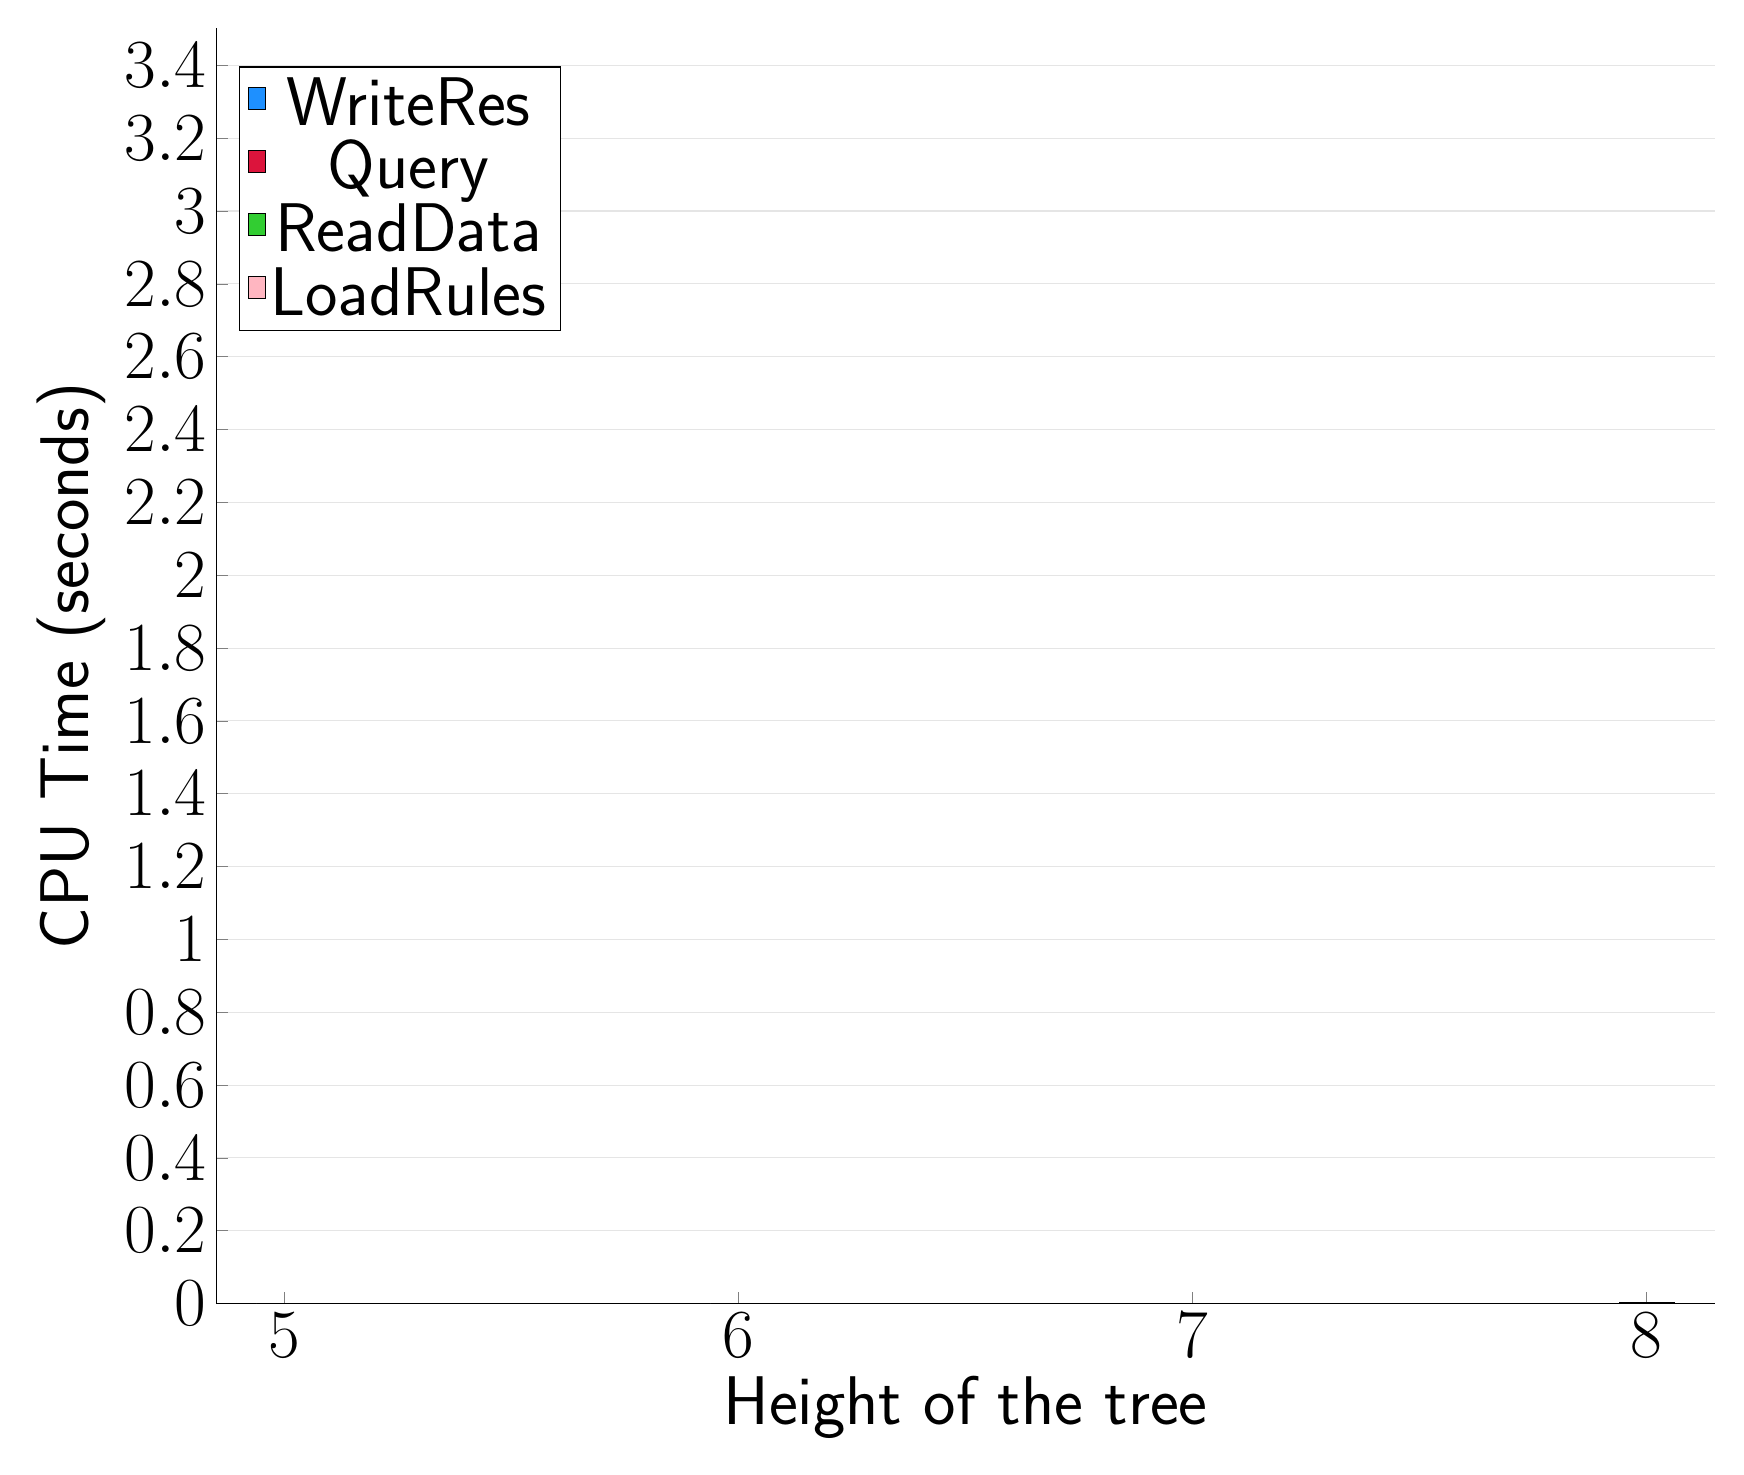
\begin{tikzpicture}
\begin{axis}[
   ybar stacked,
   width=1.7\textwidth,
   bar width=0.7cm,
   ymajorgrids, tick align=inside,
   major grid style={draw=gray!20},
   xtick=data,
   ymin=0, ymax=3.5020000000000002,
   axis x line*=bottom,
   axis y line*=left,
   enlarge x limits=0.05,
   legend style={
       at={(0.23, 0.97)},
       anchor=north east,
       legend columns=1,
       font=\Huge,
   },
   ylabel={CPU Time (seconds)},
   xlabel={Height of the tree},
   label style={font=\Huge},
   tick label style={font=\Huge},
]
\addlegendimage{fill=DodgerBlue, draw=black, line width=0.2pt}
\addlegendentry{WriteRes}
\addlegendimage{fill=Crimson, draw=black, line width=0.2pt}
\addlegendentry{Query}
\addlegendimage{fill=LimeGreen, draw=black, line width=0.2pt}
\addlegendentry{ReadData}
\addlegendimage{fill=LightPink, draw=black, line width=0.2pt}
\addlegendentry{LoadRules}
\addplot +[fill=LightPink, draw=black, line width=0.2pt] coordinates {
(5, 0.0006008000000000005)
(6, 0.0005957)
(7, 0.0006129999999999997)
(7, 0.0006053000000000005)
(7, 0.0006018999999999998)
(8, 0.0006132999999999998)
(8, 0.0005990999999999998)
(8, 0.0006050000000000007)
};
\addplot +[fill=LimeGreen, draw=black, line width=0.2pt] coordinates {
(5, 0.0001602999999999997)
(6, 0.0001879000000000004)
(7, 0.0002433000000000004)
(7, 0.00023979999999999978)
(7, 0.00023679999999999977)
(8, 0.0003601999999999996)
(8, 0.00035109999999999964)
(8, 0.0003507999999999996)
};
\addplot +[fill=Crimson, draw=black, line width=0.2pt] coordinates {
(5, 1.8999999999999916e-05)
(6, 3.479999999999992e-05)
(7, 6.669999999999993e-05)
(7, 6.76000000000003e-05)
(7, 6.659999999999982e-05)
(8, 0.00014820000000000002)
(8, 0.00014599999999999948)
(8, 0.00014980000000000033)
};
\addplot +[fill=DodgerBlue, draw=black, line width=0.2pt] coordinates {
(5, 0.0001587000000000004)
(6, 0.0003006000000000001)
(7, 0.0006444000000000002)
(7, 0.0006502999999999998)
(7, 0.0006463999999999996)
(8, 0.001449)
(8, 0.0014487000000000002)
(8, 0.0014464)
};
\end{axis}
\end{tikzpicture}

\end{document}
